\chapter{Prototyping in Office Message System}
%Introduction
This prototype exemplifies the use of Java RMI Clients and Servers. As well as showing the basics of Remote Method Invocation, a basic leader-election algorithm is implemented. This leader-election takes place if it is discovered, that the current leader has gone down.

In the prototype the leader, and only the leader, will register the function "GloriousLeader" on the RMI Registry. 
If the leader goes down, a new leader will be elected this will ReBind its own GloriousLeader function.

In perspective, the GloriousLeader function should access something that required a single-node access. In this basic prototype, the function returns the NodeID of the leader node as well as short message (as a String object).

\section{System setup}
\subsection{Setting up RMI Registry}
The host machine must host the RMI registry, the service in charge of serving up Remote Method calls.
The RMI Registry uses the CLASSPATH variable to identify the Java classes/methods bound and requested from the host. 

Therefore, the CLASSPATH variable must be set:

\begin{center}
	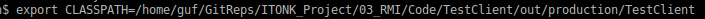
\includegraphics[width=\textwidth]{ExportingClasspath.png}
	\captionof{figure}{Exporting the CLASSPATH variable on Linux}
\end{center}

This is the path to the base directory of the .class files, compiled with the Java Compiler (Through IntelliJ).

When this is done, the RMI registry is started by the command:

\textit{rmiregistry \&}

\subsection{Running the Servers}
When starting the main programs, java needs to know the path to the .class files of the project. The java.rmi.server also needs to know the path to the actual .class files.

This is done through:
[INSERT PICTURE OF STARTING MAIN PROGRAMS]

\section{System description}
The system consists of nodes in a ring-like configuration.

Each node can be either a leader or a slave Node. 
\subsection{Node}
The node is the main entity in the system. Each node has the capacity for being both leader and slave. 

All nodes has a Server and a Client object. After a leader election, if a Node declares itself the leader, it will create a LeaderClass object for itself. 

The Node class exposes methods for interacting with the Server and Client objects.

\subsubsection{Hello Interface}

\subsubsection{Server}
The Server object takes care binding and serving up functions. The Server implements the Hello interface. 

[INSERT BDD OF SERVER]

When the Server comes online it registers itself to the RMI registry with id "QuestNodeXX" where XX is the ID of the node, that owns the Server. This is done in the servers constructor:

\begin{center}
	\fbox{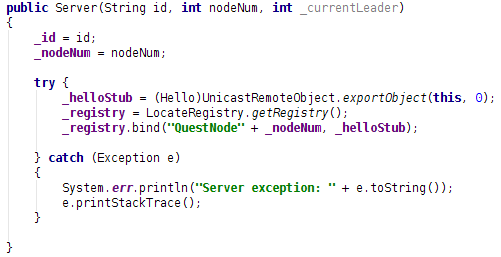
\includegraphics[width=\textwidth]{ServerConstructor.png}}
	\captionof{figure}{Constructor for the Server class}
\end{center}


The main purpose of the Server is to expose:

\begin{itemize}
\item Questing Methods for leader elections
\item OrganizationMessage(\textit{int leaderID})
\end{itemize}

If the node is Leader, the Server owns a LeaderClass object that exposes the GloriousLeader function. 

\subsubsection{Client}
The Client class is the entity in charge of calling the GloriousLeader function, after looking up the RMI registry.

The CallGloriousLeader() makes a lookup in the RMI registry, to find the leader function. It calls the function and prints the response.

\begin{center}
	\fbox{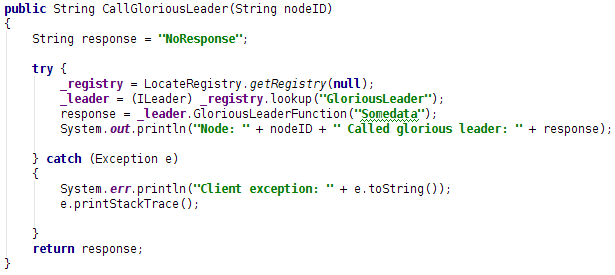
\includegraphics[width=\textwidth]{ClientCallGloriousLeader.png}}
	\captionof{figure}{CallGloriousLeader in the Client class}
\end{center}

\subsubsection{ILeader}
The ILeader interface is the interface for the Leader and exposes the GloriousLeader function. This interface is used to create the RMI stub of the LeaderClass in the Client objects.

\begin{center}
	\fbox{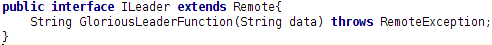
\includegraphics[width=\textwidth]{ILeaderInterface.PNG}}
	\captionof{figure}{The ILeader interface definition}
\end{center}

The GloriousLeader function throws the RemoteException if something goes wrong. This is strictly necessary to detect when something goes wrong in the transmission and a leader election is necessary.

\subsubsection{LeaderClass}
This is the implementation of the ILeader interface. This class is created when a Node is elected leader.

Upon creation, the LeaderClass checks, if the "GloriousLeader" id is found in the RMI registry. If it is found it will be unbound by the Registry.UnBind(String) function. 

The LeaderClass will then rebind itself as the "GloriousLeader", so that the current Node is now in charge of the GloriousLeader function.

\begin{center}
	\fbox{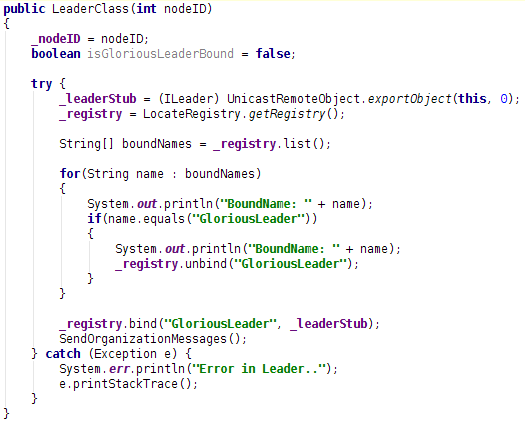
\includegraphics[scale=1]{LeaderClassConstructor.png}}
	\captionof{figure}{The LeaderClass Constructor}
\end{center}

When the new leader is bound, it will send out organization messages with the new leader ID, using the SendOrganizationMessages function.

\subsection{System}
%Description of the system with nodes in different processes etc.
%This might be removed and a system description moved i

\section{Leader Election}
\subsection{Purpose}
\subsection{GloriousLeader function}
\subsection{Bully implementation}
\subsubsection{[QUESTING FUNCTION]}
\subsection{Ring implementation}
\subsubsection{[QUESTING FUNCTION]}
\subsection{Optimized Bully}
\subsubsection{QuestingFunction}




\begin{center}
	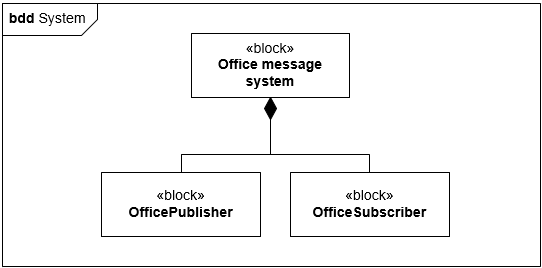
\includegraphics[width=\textwidth]{bdd_image.png}
	\captionof{figure}{BDD of the Office Message System}
\end{center}
\section{Tests}